% v2-acmtog-sample.tex, dated March 7 2012
% This is a sample file for ACM Transactions on Graphics
%
% Compilation using 'acmtog.cls' - version 1.2 (March 2012), Aptara Inc.
% (c) 2010 Association for Computing Machinery (ACM)
%
% Questions/Suggestions/Feedback should be addressed to => "acmtexsupport@aptaracorp.com".
% Users can also go through the FAQs available on the journal's submission webpage.
%
% Steps to compile: latex, bibtex, latex latex
%
% For tracking purposes => this is v1.2 - March 2012
\documentclass{acmtog} % V1.2

%\acmVolume{VV}
%\acmNumber{N}
%\acmYear{YYYY}
%\acmMonth{Month}
%\acmArticleNum{XXX}
%\acmdoi{10.1145/XXXXXXX.YYYYYYY}

\acmVolume{1}
\acmNumber{1}
\acmYear{2017}
\acmMonth{November}
\acmArticleNum{1}
\usepackage{float}
\usepackage{graphicx}
\usepackage{amsmath}
\usepackage{listings}
\usepackage{amssymb}


% Copyright
\setcopyright{rightsretained}


\begin{document}

\markboth{V. F. Pamplona et al.}{Photorealistic Models for Pupil Light Reflex and Iridal Pattern Deformation}

\title{Report of Chapter 8 \& 9} % title

\author{Qifeng Lin \\ 17214656}
% NOTE! Affiliations placed here should be for the institution where the
%       BULK of the research was done. If the author has gone to a new
%       institution, before publication, the (above) affiliation should NOT be changed.
%       The authors 'current' address may be given in the "Author's addresses:" block (below).
%       So for example, Mr. Fogarty, the bulk of the research was done at UIUC, and he is
%       currently affiliated with NASA.


\maketitle


\section{Review}
    Chapter 8 mainly talks about liveness properties and chapter 9 mainly demonstrate deadlock-freeness.

    Firstly, a liveness property states that some event will ultimately occur under certain conditions. For example, "the light will turn green" can be seen as a liveness property. And it should be noted that liveness properties mean that something happens but not that properties of being live. Being live states that all components of the system remain reachable.

    In chapter 8, it devotes to stating simple liveness. In temporal logic, simple liveness exists in \textbf{F} combinator and \textbf{U} combinator because \textbf{F} combinator naturally includes the meaning of eventual occurrence and $P\textbf{U}Q$ guarantees the occurrence of $Q$, which means that something will ultimately happen under certain conditions and exactly the meaning of liveness properties. However, \textbf{W} combinator cannot be used to express liveness properties since $P\textbf{W}Q$ does not guarantee the occurrence of $Q$.

    We have introduced the notion of liveness properties and need to explain the usage of them. It leads to a discussion about weather liveness properties if useful. Here, liveness properties are divided into two class: "abstract" and "bounded" liveness properties. Abstract liveness properties states that something will eventually occur and bounded liveness properties are constrained with time or other conditions. It can be seen as discussion of "abstract" and "concrete". Compared with "concrete", "abstract" is more general and efficient. But they are not contradictory because if "abstract" is not fulfilled, neither "concrete".

    Since we need to apply liveness in the model, we should figure out how to find liveness in models. In this way, we speak of liveness hypotheses. Firstly, we investigate the liveness hypotheses which implicitly occur in the models. For example, a mathematical model representing a real system incorporates implicit safety and liveness hypotheses. The implicit safety means that a state moves to another state only if it includes the corresponding transition. As for implicit liveness hypotheses, it means that the system does not terminate without reason or that the system does not remain inactive indefinitely without reason. Take Fig.1 as an example.
    \begin{figure}[H]
      \centering
      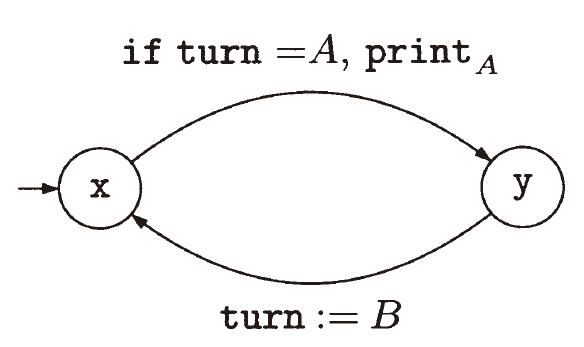
\includegraphics[width=2.0in]{1.jpg}
      \caption{The user A}
    \end{figure}

    The automaton in state x can print only if $\textbf{turn} = A$, otherwise remain in state x. And in state y, the system ends up returning to state x by assigning $B$ to \textbf{turn}. Obviously, the hypothesis that in state x the system can end up printing, is a liveness hypothesis. But in reality, user A does not necessarily operate in this way and the system remain inactive indefinitely. It can be seen as the result of difference of reality and the system. Therefore, we can see that it is difficult to find all the premises and to check if they can be satisfied.

    Also, sometimes, it can not incorporate the liveness hypotheses which seem necessary into a given model. Take Fig.2 as an example.
    \begin{figure}[H]
      \centering
      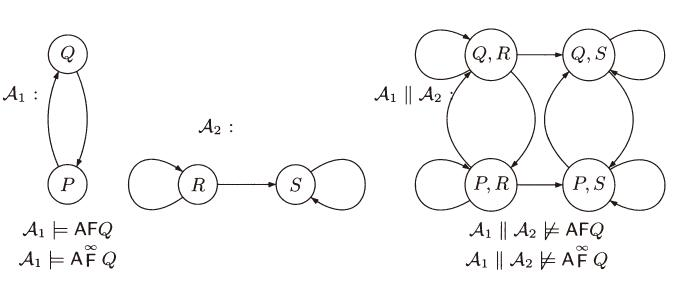
\includegraphics[width=3.5in]{2.jpg}
      \caption{The liveness of $\mathcal{A}_1$ does not carry over to $\mathcal{A}_1||$$\mathcal{A}_2$}
    \end{figure}
    
    In Fig.2, we can see that in the automaton $\mathcal{A}_1$, $Q$ is unavoidable. we can write it in $\mathcal{A}_1\models\textbf{AF}Q$ or$\mathcal{A}_1\models\textbf{A}\overset{\infty}{\textbf{F}} Q$. But if we compose $\mathcal{A}_1$ asynchronously with $\mathcal{A}_2$, the property is no longer ensured. It means that the liveness satisfied in automaton $\mathcal{A}_1$ cannot hold in composed automaton.
    
    We have mentioned a case where there exists a mismatch between the real system behavior and the liveness hypotheses. Under the condition, we can apply verification only if:
    \begin{itemize}
      \item the liveness hypotheses of the model must be less constraining than the desired liveness hypothesis
      \item the temporal logic must be rich enough to express the liveness hypotheses that are not guaranteed by the model.
    \end{itemize}
    
    It leads to the specific model behaviors which hold the liveness hypothesis ($\phi_v$). And we can express it satisfies a given property $\psi$ as $\phi_v\Rightarrow\psi$.
    
    Previously, we have talked about the abstract liveness and here we have a discussion about Bounded Liveness. A bounded Liveness property means that a liveness property that comes with a maximal delay within which the "desired situation" must occur. Therefore, it is usually regarded as a safety property. And techniques applied to safety properties can be applied to bounded liveness properties.

    At last, we talked about deadlock-freeness. Deadlock-freeness is a special property, stating that the system can never be in a situation in which no progress is possible. And in general, it is expressed as $\textbf{AGEX true}$ in CTL, which means that whatever the state reached may be \textbf(AG), there will exist an immediate successor state (\textbf{EX true})". It is obvious that the expression excludes deadlock because the system won't remain inactive and no progress is possible.
    
    Deadlock-freeness cannot be regarded as a simple safety property as we can see that the expression of deadlock-freeness is not in the form of $\textbf{AG}\phi^-$. But we need to understand how verify deadlock-freeness. We often express that the system cannot reached a undesired condition. Take Fig.3 as an example.
    \begin{figure}[H]
      \centering
      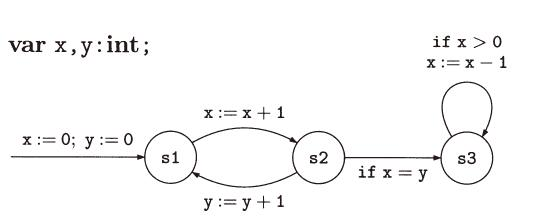
\includegraphics[width=3.5in]{3.jpg}
      \caption{$\mathcal{A}$: A deadlock-free system}
    \end{figure}
    
    Obviously, the deadlock-freeness is expressed as the following formula:
    \begin{equation*}
      \mathcal{A}\models\textbf{AG}\neg(\text{s3}\wedge\text{x}\leq0)
    \end{equation*}
    
    If we delete some transitions of $\mathcal{A}$, the resulted automaton no longer hold deadlock-freenes. The result is as Fig.4 shows.
    \begin{figure}[H]
      \centering
      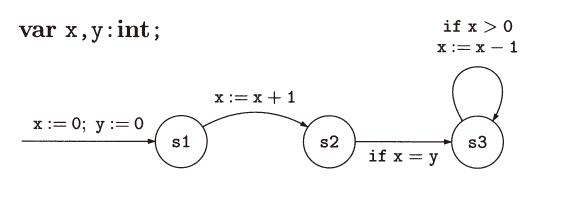
\includegraphics[width=3.5in]{4.jpg}
      \caption{$\mathcal{A}'$: A variant of the previous example}
    \end{figure}
    
    But what about add some transitions? Actually, even if the system we obtain is deadlock-free, this does not guarantee that the initial system was.
    
\section{Summary}
    Chapter 8 and chapter 9 demonstrate liveness properties and deadlock-freeness. For liveness properties, it is useful to verify if what we want will occur and deadlock-freeness help us to ensure the correctness of the system. 



\end{document}
% End of v2-acmtog-sample.tex (March 2012) - Gerry Murray, ACM
